% !TEX TS-program = xelatex
% !BIB TS-program = bibtex
\documentclass[12pt,letterpaper]{article}
\usepackage{style/dsc180reportstyle} % import dsc180reportstyle.sty

%%%%%%%%%%%%%%%%%%%%%%%%%%%%%%%%%%%%%%%%%%%%%%%%%%%%%%%%
%%%% Title and Authors
%%%%%%%%%%%%%%%%%%%%%%%%%%%%%%%%%%%%%%%%%%%%%%%%%%%%%%%%

\title{Predicting Financial Transaction Categories: A Comparative Analysis of Machine Learning Based Methods for Optimal Classification}

\author{
\begin{tabular}[t]{ccc}
Brandon Dioneda & Mert Ozer & Qianjin Zhou \\
{\tt bdioneda@ucsd.edu} & {\tt mozer@ucsd.edu} & {\tt q9zhou@ucsd.edu}
\end{tabular}
\\[4ex]
\begin{tabular}[t]{ccc}
Brian Duke (Mentor) & Kyle Nero (Mentor) & Berk Ustun (Mentor)\\
{\tt brian.duke@prismdata.com} & {\tt kyle.nero@prismdata.com} & {\tt berk@ucsd.edu}
\end{tabular}
}

\begin{document}
\maketitle

%%%%%%%%%%%%%%%%%%%%%%%%%%%%%%%%%%%%%%%%%%%%%%%%%%%%%%%%
%%%% Abstract and Links
%%%%%%%%%%%%%%%%%%%%%%%%%%%%%%%%%%%%%%%%%%%%%%%%%%%%%%%%


\begin{abstract}
    \textcolor{LightGrey}{Evaluating creditworthiness has been a challenge since the 19th century, with FICO scores becoming the most widely used metric today. However, traditional credit scoring models often overlook consumers who lack conventional credit history, leading to unequal access to credit. With the advent of digital technology, alternative data sources now offer the opportunity for more inclusive credit assessments. This project addresses these gaps by analyzing non-personal financial information, such as categorizing bank transactions and predicting personal income to assess creditworthiness more fairly.}
\end{abstract}

\begin{center}
Code: \url{https://github.com/mozer123/credit_score/}
\end{center}

\maketoc
\clearpage

%%%%%%%%%%%%%%%%%%%%%%%%%%%%%%%%%%%%%%%%%%%%%%%%%%%%%%%%
%%%% Main Contents
%%%%%%%%%%%%%%%%%%%%%%%%%%%%%%%%%%%%%%%%%%%%%%%%%%%%%%%%

\section{Introduction}
\subsection{Background Information}
    {Creditworthiness assessment has been a longstanding challenge, and while modern credit scores became widely adopted in 1989, these traditional models often fail to account for the financial profiles of individuals who lack conventional credit histories. As a result, millions are excluded from fair access to credit. Moreover, early credit evaluations were frequently marred by discriminatory practices, factoring in age, race, and marital status, while even today, reliance on conventional credit history can reinforce socioeconomic biases. 

    This project leverages bank data from 2017-2023 to develop a fairer, non-discriminatory model for assessing credit risk. By categorizing individual bank transactions and predicting personal income as alternative indicators, our approach emphasizes unbiased and responsible credit assessments, aiming to expand equal access to credit.
    }
\subsection{Literature Review and Discussion of Prior Work}
    {In their review, Markov, Seleznyova, and Lapshin (2022) discuss the evolving trends in credit scoring methodologies, highlighting the shift from traditional statistical methods, such as logistic regression, toward more complex machine learning models, including decision trees, neural networks, and ensemble methods. The authors emphasize the growing popularity of explainable AI (XAI) in credit scoring, as financial institutions are required to provide transparency in their decision-making processes, especially in highly regulated environments. They also underscore the importance of considering biases in model training, especially when alternative data sources are involved, as biased data can lead to discriminatory credit outcomes. This work sets the stage for understanding the inherent challenges in balancing model accuracy and fairness, particularly when advanced techniques are employed.
        
    Litty (2024) explores the integration of alternative data sources, such as social media behavior, mobile phone usage patterns, and even psychometric data, in credit risk assessment models. These sources offer the potential to improve credit scoring accuracy, especially for individuals with limited or no traditional credit history, thus addressing the issue of financial inclusion. Litty’s work outlines the effectiveness of AI-powered models in capturing complex relationships within these unstructured data sources, which are often ignored in conventional credit scoring models. Furthermore, Litty’s research identifies the potential risks of privacy invasion and data security when using personal and behavioral data, suggesting that such risks must be carefully managed to avoid ethical concerns.
    
    Together, these studies highlight the transformative role of AI in credit scoring, offering insights into both the benefits and challenges of these new methods. Unlike traditional models that rely on static financial data, our approach leverages natural language processing (NLP) on transaction memos and additional data sources to develop a more holistic view of consumer behavior. By focusing on these unstructured transaction details, we aim to extract latent features that may reveal patterns of financial responsibility not captured in traditional scoring systems. This approach not only improves the granularity of credit assessment but also offers a pathway to more personalized credit models, contributing to ongoing efforts in making credit scoring more inclusive and responsive to diverse financial behaviors.
    }
    
\subsection{Description of Relevant Data}
{Data provided by PrismData which are bank transactions that are from customers that use PrismData credit products from years 2017-2023:}
\begin{itemize}
    \item {Inflows.pqt: Contains transaction-level information on inflowing transactions (such as: paychecks, refunds, etc.)}
    \begin{figure}[H]
        \centering
        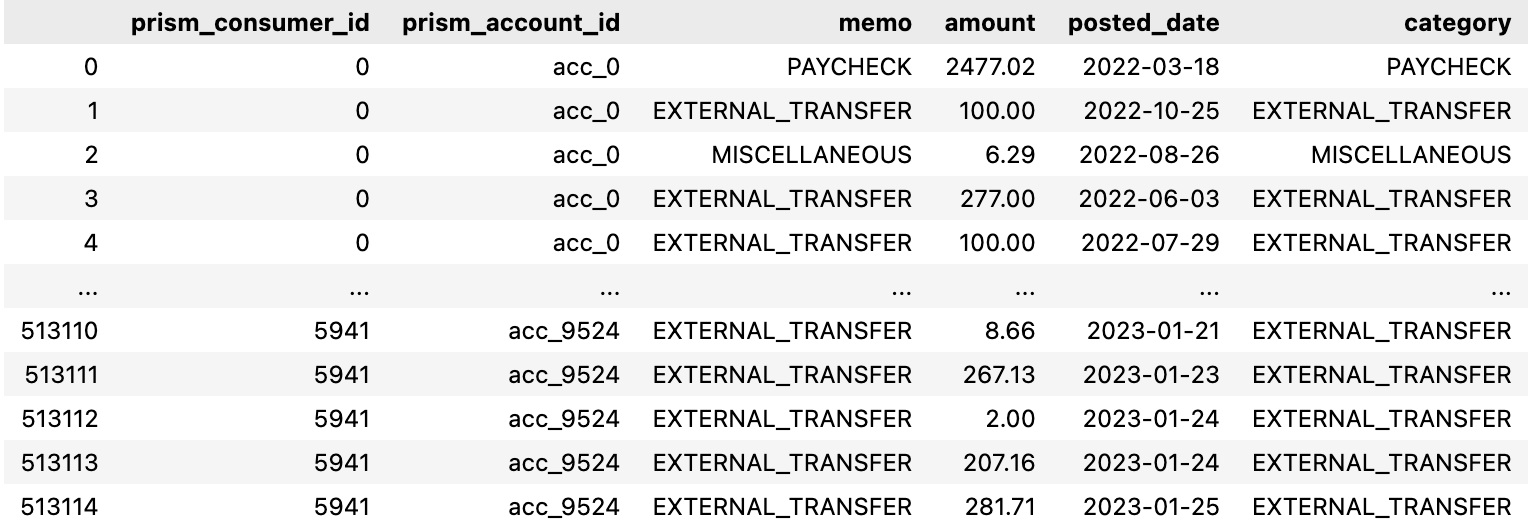
\includegraphics[width=0.6\textwidth]{pngs/inflows.png}
        \caption{Inflows.pqt}
        \label{fig:enter-label}
    \end{figure}
    
    \item {Outflows.pqt: Contains transaction-level information on outflowing transactions (such as: groceries, rent, etc.)}
    \begin{figure}[H]
        \centering
        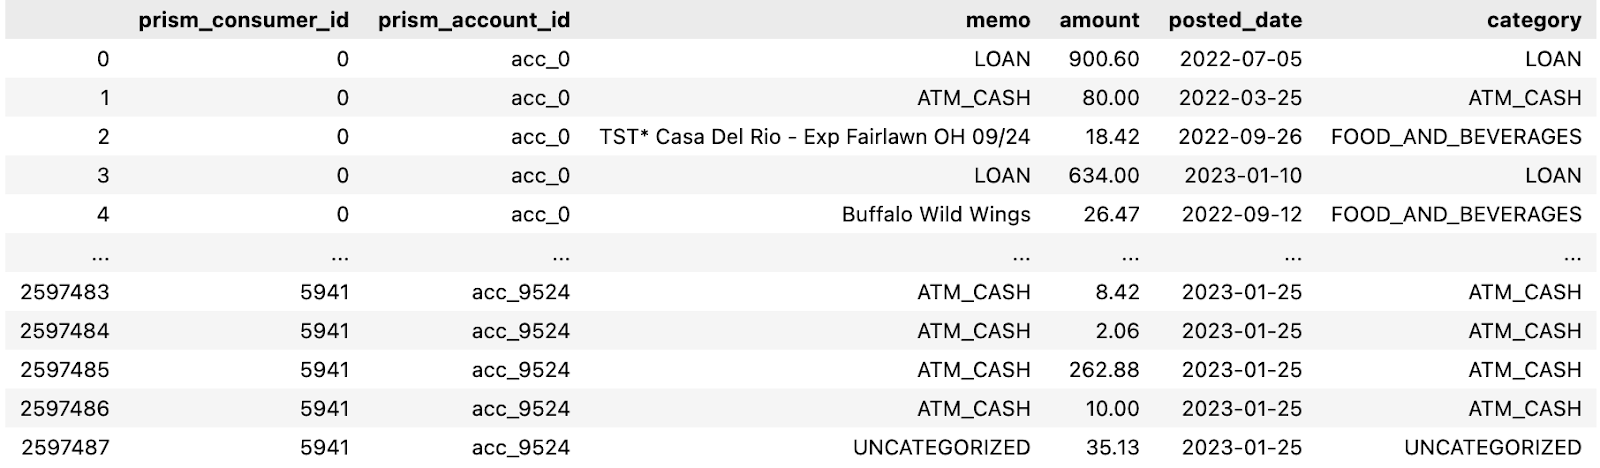
\includegraphics[width=0.6\textwidth]{pngs/outflows.png}
        \caption{Outflows.pqt}
        \label{fig:enter-label}
    \end{figure}
    
\end{itemize}
Columns:
\begin{itemize}
    \item {prism\_consumer\_id: ID associated with the consumer}
    \item {prism\_account\_id: ID associated with the account}
    \item {memo: Descriptive text for the transaction}
    \item {amount: Transaction amount}
    \item {posted\_date: Date when the transaction was posted}
    \item {category: Type/category of the transaction}
\end{itemize}

\section{Methods}
\subsection{Exploratory Data Analysis and Bias Checking}
\begin{enumerate}
    \item{\textbf{Summary Statistics of Transaction Amounts:}
    
    The variable (transaction) "amount” is important information that could potentially help us build our models, hence we calculated the summary statistics of “amount” for both inflow and outflow datasets.}
    \begin{itemize}
        \item {Inflow Data:}
            \begin{itemize}
                \item{Count: 513,115 transactions}
                \item{Mean amount: \$734.70}
                \item{Median amount: \$100.00}
                \item{Standard deviation: \$5,296.57}
                \item{Range: \$0.01 to \$1,154,966.00}
            \end{itemize}
    
        \item {Outflow Data:}
            \begin{itemize}
                \item{Count: 2,597,488 transactions}
                \item{Mean amount: \$145.13}
                \item{Median amount: \$24.26}
                \item{Standard deviation: \$1,697.88}
                \item{Range: \$0.00 to \$654,853.20}
            \end{itemize}
    \end{itemize}
{As shown in the summary statistics above,  inflows tend to have higher transaction amounts compared to outflows, with a significant difference in mean and maximum values.}

    \item{\textbf{Category Distribution:}}
    \begin{figure}[H]
        \centering
        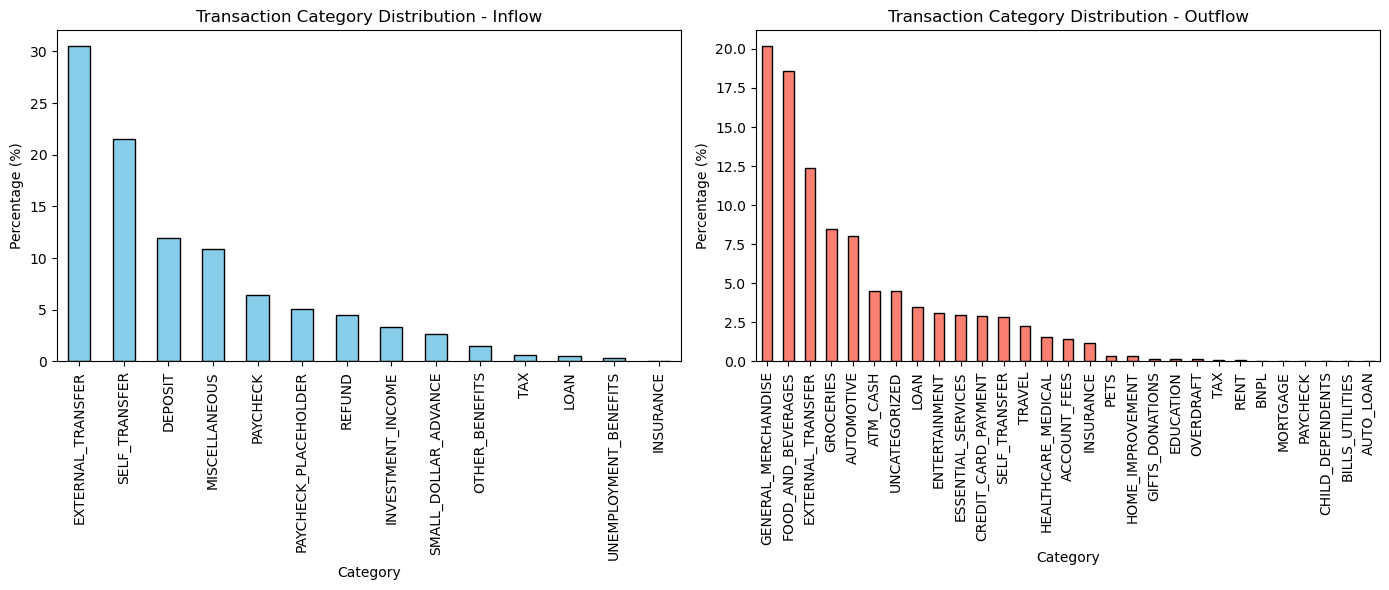
\includegraphics[width=1.0\textwidth]{pngs/category_dist.png}
        \caption{Category Distribution}
        \label{fig:enter-label}
    \end{figure}
    \begin{itemize}
        \item Inflow Data: Most common categories are EXTERNAL\_TRANSFER $(30.5\%)$ and SELF\_TRANSFER $(21.5\%)$.
        \item Outflow Data: Most common categories are GENERAL\_MERCHANDISE $(20.2\%)$, FOOD\_AND\_BEVERAGES $(18.6\%)$, and EXTERNAL\_TRANSFER $(12.4\%)$.
    \end{itemize}

    {We also computed the most common merchants(“memo”) per category for both outflow and inflow dataset. The results for the inflow dataset are not displayed because all memos exactly match their categories.}
    \begin{figure}[H]
        \centering
        \includegraphics[width=0.4\textwidth]{pngs/fig_3.png}
        \caption{Most Common Merchant per Category - Outflow Dataset}
        \label{fig:enter-label}
    \end{figure}
    {From Figure 4 we can see that McDonald’s, Amazon, Walmart, Uber, etc. are the most common merchants for each category they belong to. It is worth noting that the process of finding the most common merchant is based on the uncleaned “memo” column.}
\end{enumerate}

\subsection{Cleaning Memo}
Here is how we cleaned the memo and various considerations.

\begin{itemize}
    \item Filtered rows where the memo field differs from the category field 
    \item The resulting unique categories are: ['FOOD\_AND\_BEVERAGES', 'GENERAL\_MERCHANDISE', 'GROCERIES', 'PETS', 'TRAVEL', 'MORTGAGE', 'OVERDRAFT', 'EDUCATION', 'RENT']
    \item Converted memo to lowercase
    \item Removed special characters and numbers to focus on text-based features
    \item Removed placeholders (e.g., sequences like "xxx")
    \item Trimmed extra spaces to clean up the text field further
\end{itemize}
\begin{figure}[H]
    \centering
    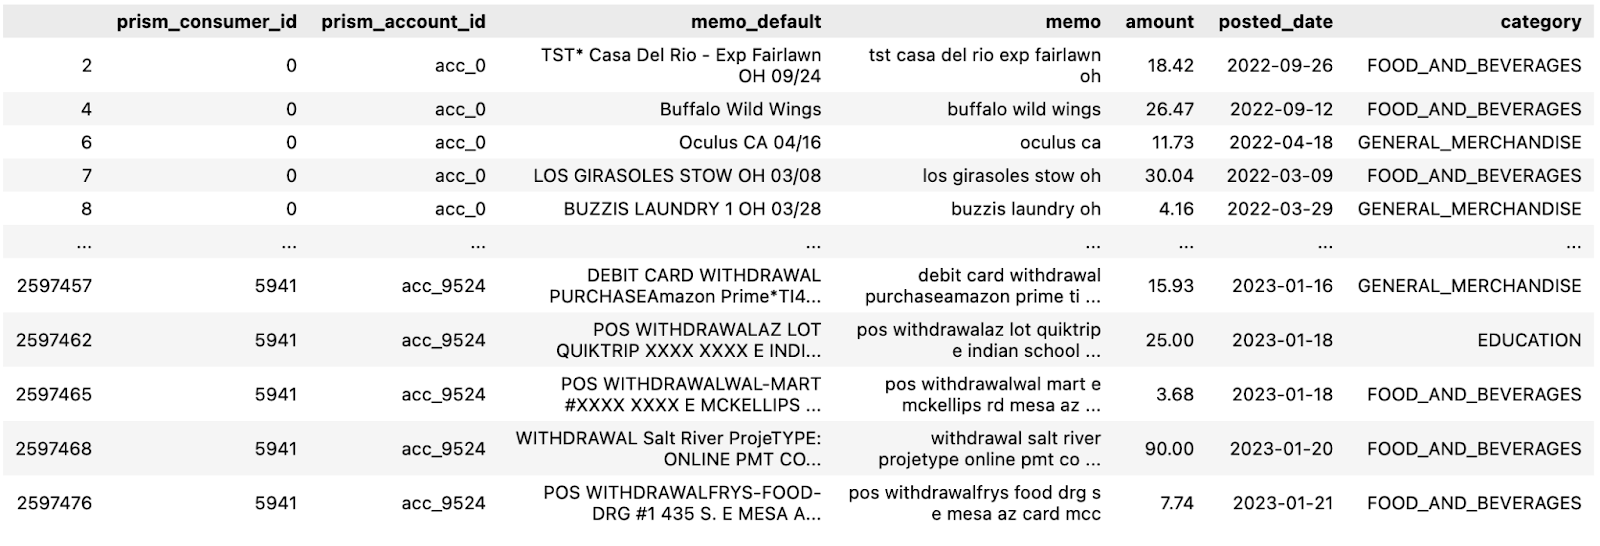
\includegraphics[width=1.0\textwidth]{pngs/memo_clean.png}
    \caption{Original Memos vs Cleaned Memos}
    \label{fig:enter-label}
\end{figure}

\subsection{Categorization Approaches}
These are the various methods we tried.

\section{Results}
\subsection{tfidf+svm}
Confusion matrix and accuracy of each method. Testing conditions and environments. Inference and training times.
\subsection{other method}

\section{Discussion}
\subsection{Summary of Methods}
Table summarizing all factors in choosing the best method.

Table \ref{tab:sometab1} presents some summary of the data.

\begin{table}[htbp]
\caption{Some Table Caption}
\label{tab:sometab1}
\resizebox{0.4\linewidth}{!}{\input{table/sometab1}}
\end{table}

Table \ref{tab:sometab2} presents some summaries of the performance of our model.

\begin{table}[htbp]
\caption{Some Other Table Caption}
\label{tab:sometab2}
\resizebox{0.9\linewidth}{!}{\input{table/sometab2}}
\end{table}

\subsection{}
This is the best model overall
but these are also useful in these constraints.

\section{Conclusion}

\subsection{Inline Citation Examples}

Citation in text (no parentheses): use \texttt{{\textbackslash}cite\{citekey\}}. 
For example, \cite{breiman2011}, \cite{devlin2019bert}.

Citation in parentheses: use \texttt{{\textbackslash}citep\{citekey\}}. 
For example: \citep{vaswani2023attention}, \citep{karras2019stylebased}.


%%%%%%%%%%%%%%%%%%%%%%%%%%%%%%%%%%%%%%%%%%%%%%%%%%%%%%%%
%%%% Reference / Bibliography
%%%%%%%%%%%%%%%%%%%%%%%%%%%%%%%%%%%%%%%%%%%%%%%%%%%%%%%%

\makereference

{\color{blue} To edit the contents of the ``References" section, edit \texttt{reference.bib}. Many conference websites format citations in BibTeX that you can copy into \texttt{reference.bib} directly; you can also search for the paper on Google Scholar, click ``Cite", and then click ``BibTeX" (\href{https://scholar.google.com/scholar?hl=en&as_sdt=0%2C23&q=attention+is+all+you+need&btnG=#d=gs_cit&t=1700436667623&u=%2Fscholar%3Fq%3Dinfo%3A5Gohgn6QFikJ%3Ascholar.google.com%2F%26output%3Dcite%26scirp%3D0%26hl%3Den}{here}'s an example).}

\bibliography{reference}
\bibliographystyle{style/dsc180bibstyle}

%%%%%%%%%%%%%%%%%%%%%%%%%%%%%%%%%%%%%%%%%%%%%%%%%%%%%%%%
%%%% Appendix
%%%%%%%%%%%%%%%%%%%%%%%%%%%%%%%%%%%%%%%%%%%%%%%%%%%%%%%%

\clearpage
\makeappendix

\subsection{Training Details}

\subsection{Additional Figures}

\subsection{Additional Tables}


\end{document}